\documentclass[a4paper]{article}

\usepackage[english]{babel}
\usepackage[utf8x]{inputenc}
\usepackage{graphicx}
\usepackage{fancyhdr} %Package to configure headings and footer
\usepackage{lastpage} %Needed to display last page (total amount of pages)
\usepackage{listings}

% pagelayout
\usepackage[
top    = 2.75cm,
bottom = 2.00cm,
left   = 2.50cm,
right  = 2.00cm]{geometry}
\setcounter{secnumdepth}{4}

% header
\pagestyle{fancy}
\fancyhead[L]{\today}
\fancyhead[R]{DBSync - DezSys}

%footer
\fancyfoot[L]{Aly, Haidn}
\fancyfoot[C]{5A HIT}
\fancyfoot[R]{Seite \thepage/\pageref{LastPage}}

%title page
\author{Ahmed Aly, Martin Haidn}
\title{Synchronisation von heterogenen Datenbanken\\SYT - 5A HIT}
\date{\today}

\begin{document}
	\maketitle
	\tableofcontents
	
	\newpage
	\section{Aufgabenstellung}
	Dokumentieren Sie Ihren Versuch zwei heterogene Datenbanksysteme (MySQL, Postgresql) zu synchronisieren. Verwenden Sie dabei unterschiedliche Schemata (verschiedene Tabellenstruktur) und zeigen Sie auf, welche Schwierigkeiten bei den unterschiedlichen Heterogenitätsgraden auftreten können (wie im Unterricht besprochen) [2Pkt].\\
	\\
	Implementieren Sie eigenständig eine geeignete Middleware [8Pkt]. Testen Sie Ihr gewähltes System mit mehr als einer Tabelle 4Pkt und dokumentieren Sie die Funktionsweise, sowie auch die Problematiken bzw. nicht abgedeckte Fälle [2Pkt].\\
	\\
	Das PDF soll ausführlich beschreiben, welche Annahmen getroffen wurden. Der Source-Code muss den allgemeinen Richtlinien entsprechen und ebenfalls abgegeben werden.\\
	\\
	Gruppengröße: 2 Gesamtpunkte: 16 [Aufteilung in eckigen Klammern ersichtlich]\\
	\\
	\textbf{Punkte}\\
	\\
	Dokumentation der Synchronisation [2Pkt]\\
	\\
	Implementierung der Middleware [8Pkt]
	\begin{itemize}
		\item Zeittrigger bzw. Listener für Synchronisation bzw. DBMS Logs
		\item Konfiguration bez. Mapping der Tabellen und Attribute
		\item Konfliktlösung bei Zeitüberschneidung bzw. Datenproblemen (Log)
		\item LostUpdate-Problem\\
	\end{itemize}
	
	Test mit mehr als einer Tabelle und mindestens 10 Datensätze pro Tabelle [4Pkt]
	\begin{itemize}
		\item Uni- und Bidirektionale Änderungen mehrerer Tabellen
		\item Einfügen, Ändern und Löschen\\
	\end{itemize}
	
	Dokumenation der Funktionsweise, Problematiken und Problemfälle [2Pkt]
	\begin{itemize}
		\item Designdokumentation (Code + DB)
		\item Synchronisationsverhalten
		\item unbehandelte Problemfälle\\
	\end{itemize}
	
	Protokoll und Sourcecodedokumentation [0..-6Pkt]
	
	\newpage
	\section{Aufwandsschätzung}
	Für die Durchführung dieser Übung sind elf Stunden vorgesehen.
	Die Aufgabenstellung wurde in Arbeitsparkete untergliedert und für die jeweiligen Tasks wurde eine Zeitaufwandsschätzung erstellt.\\
	\begin{center}
		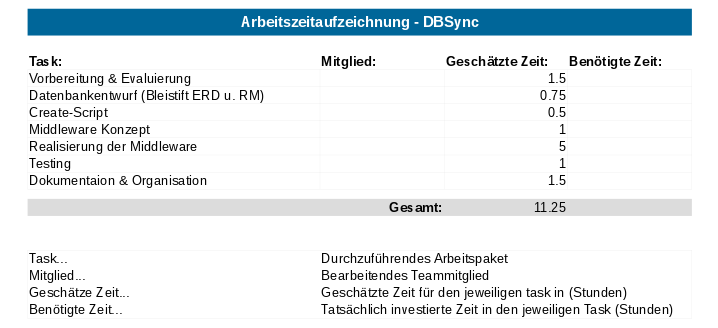
\includegraphics[width=0.8\textwidth]{img/timetable.png}
	\end{center}
	
	\section{Datenbankentwurf}
	\section{Middleware}
	\section{Arbeitsdurchführung}
\end{document}